\documentclass{article}

\usepackage{graphicx}
\usepackage{tikz}
\usepackage{tikzsymbols}
\usetikzlibrary{calc,patterns,shapes.geometric}
\pagestyle{empty}
\usepackage[margin=0pt]{geometry}
\geometry{papersize={14in,12in}}

\def\centerarc[#1](#2)(#3:#4:#5){\draw[#1] ($(#2)+({#5*cos(#3)},{#5*sin(#3)})$) arc (#3:#4:#5);}

\begin{document}
	\begin{figure}
		\centering
		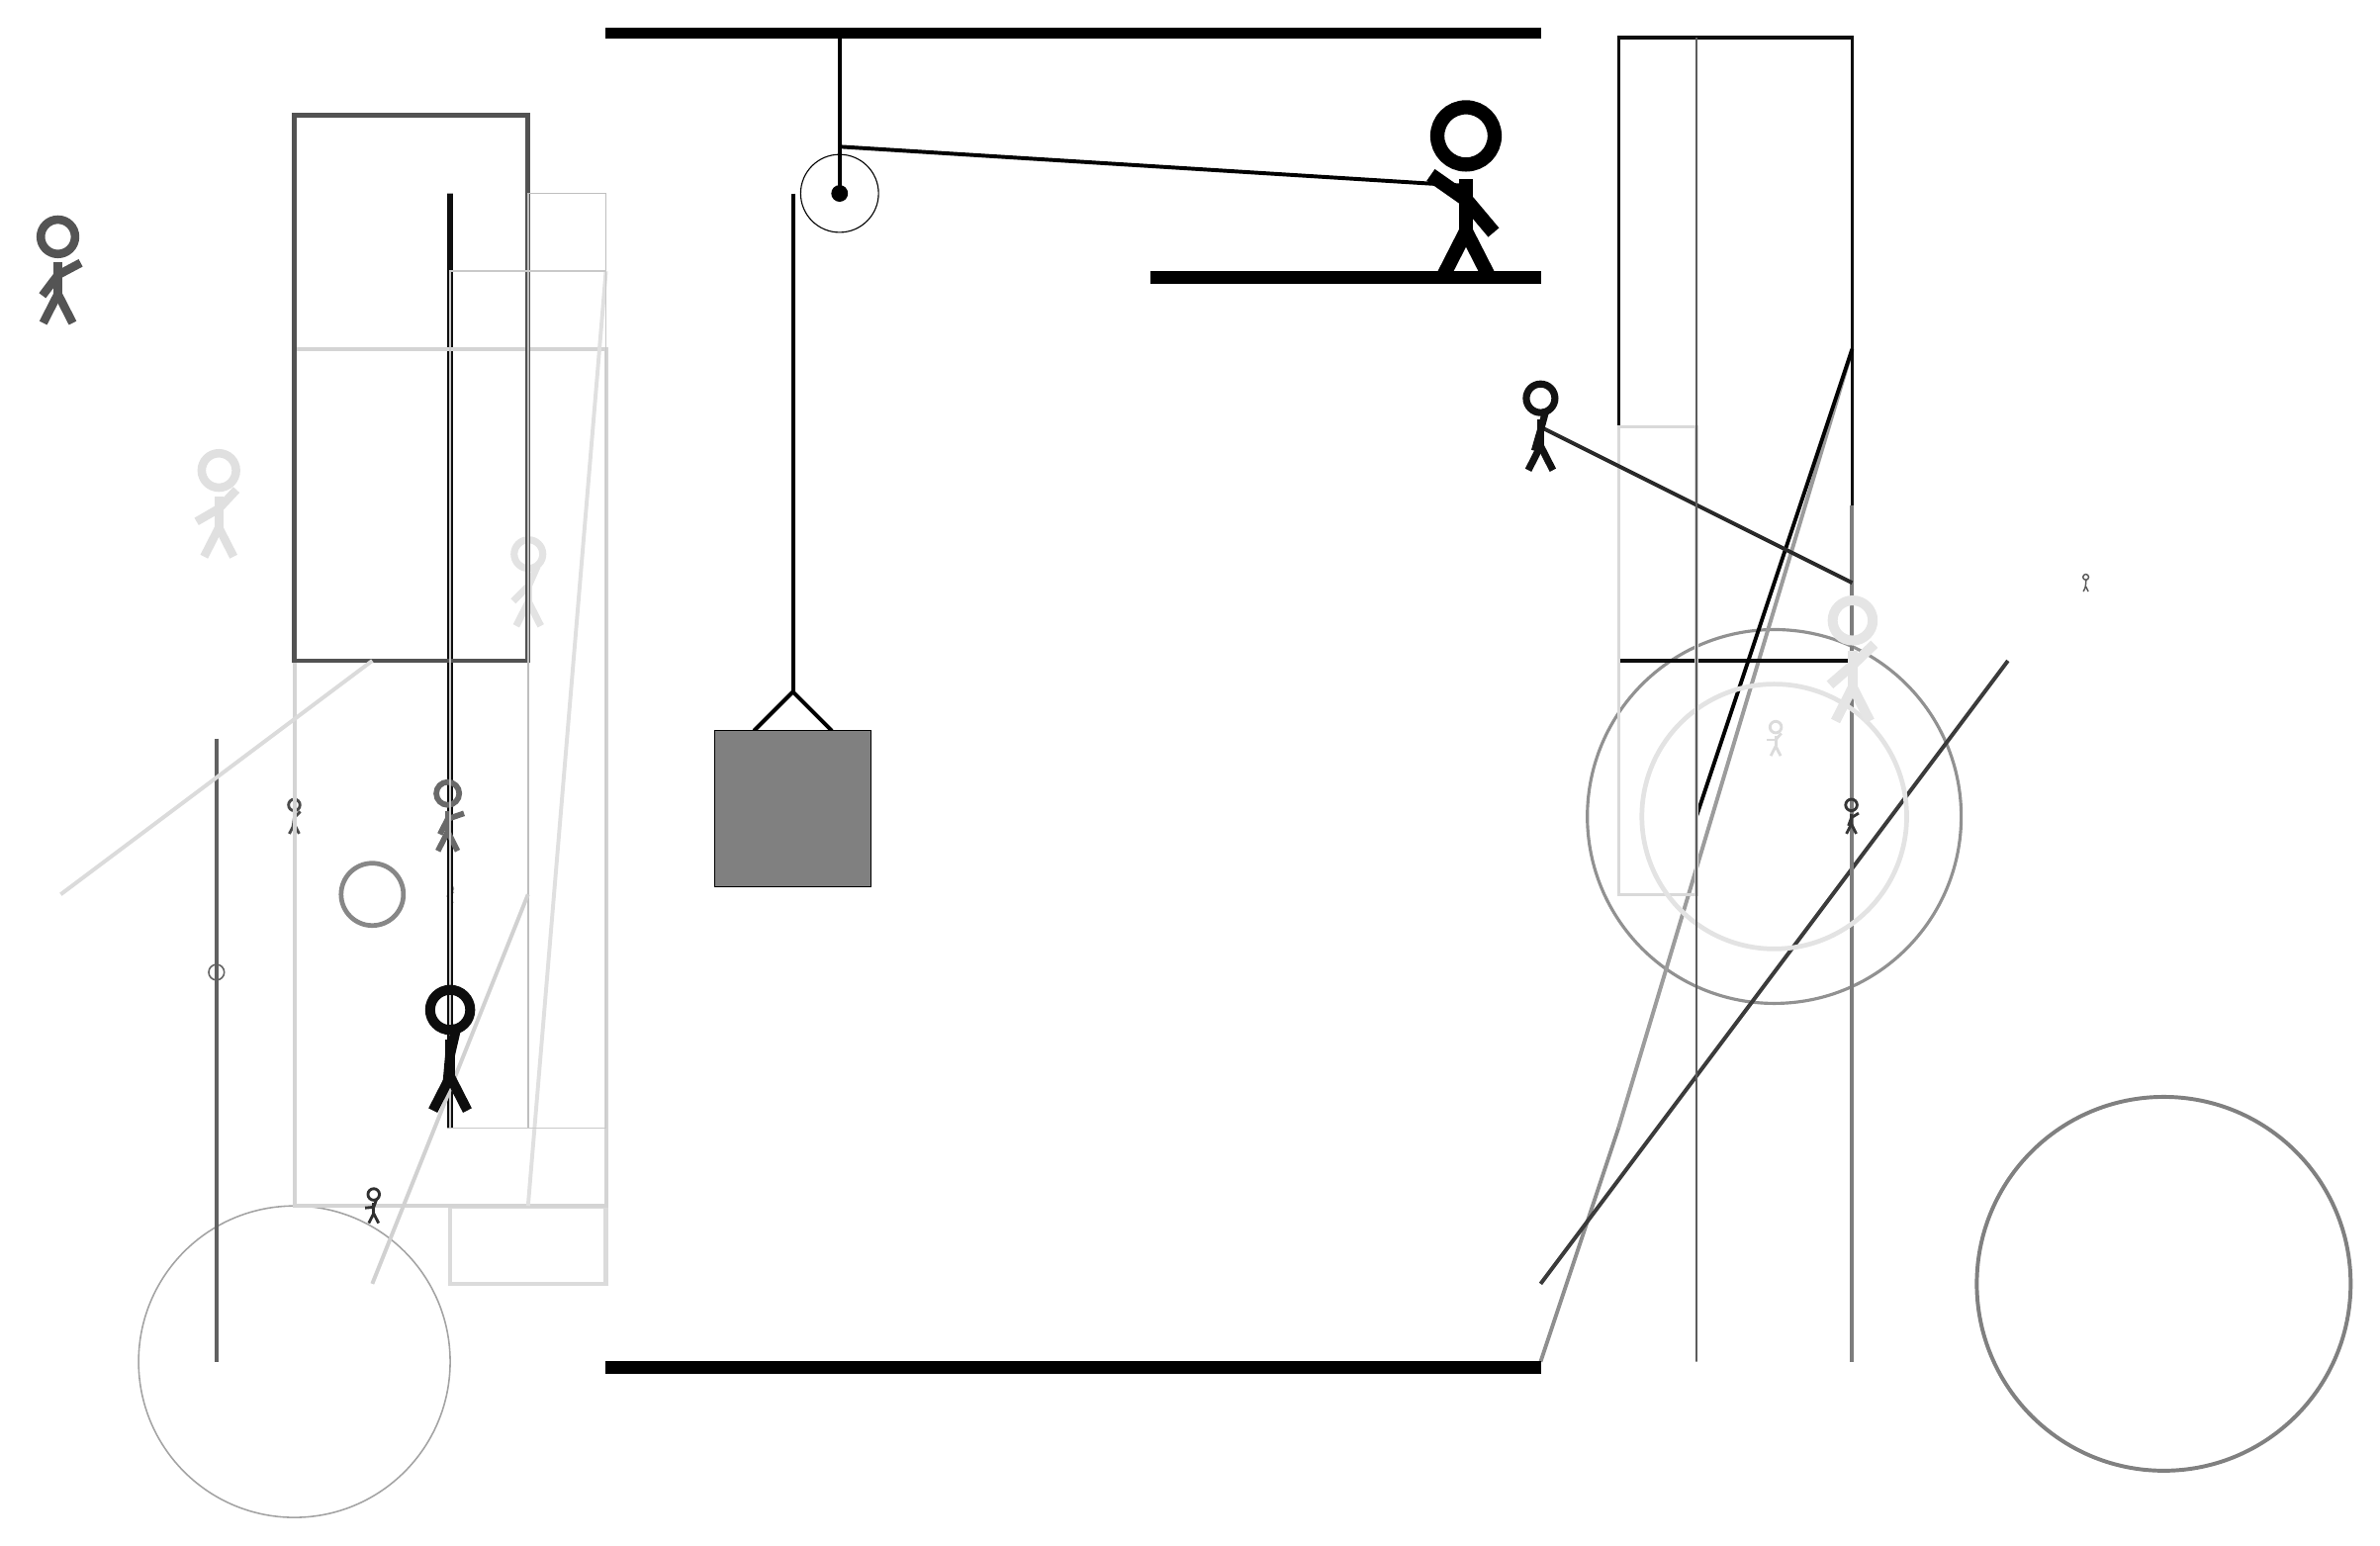
\begin{tikzpicture}
			%%%%% START %%%%%
			
			\draw[fill=black] (-2, 14) rectangle (10, 14.125);
			
			\draw (1, 12) circle (0.5);
			\draw[fill=black] (1, 12) circle (0.1);
			\draw[line width=0.5mm] (1, 14) -- (1, 12);
			
			\draw[line width=0.5mm](-0.1, 5.1) --  (0.4, 5.6) -- (0.9, 5.1);
			\draw[fill=black!50] (-0.6, 5.1) rectangle (1.4, 3.1);
			
			\draw[line width=0.5mm](0.4, 12) -- (0.4, 5.6);
			\centerarc[line width=0.5mm](1, 12)(90:180:0.6)
			\draw[line width=0.5mm](1, 12.6) -- (9, 12.1);
			
			\node[line width=0.6mm, color=black!65] at (17, 7) {\Strichmaxerl[1][83][86]};
			
			\draw [line width=0.2mm, color=black!36](-6, -3) circle (2.0);
			\node[line width=0.6mm, color=black!71] at (-6, 4) {\Strichmaxerl[2][82][46]};
			\draw [line width=0.2mm, color=black!61](-7, 2) circle (0.1);
			
			\draw[line width=0.5mm, color=black!10] (-3, 11) rectangle (-3, 7);
			\draw [line width=0.4mm, color=black!43](13, 4) circle (2.4);
			\draw[line width=0.5mm, color=black!39](14, 10) -- (11, 0);
			\draw[line width=0.5mm, color=black!44](11, 0) -- (10, -3);
			\draw[line width=0.5mm, color=black!77](10, -2) -- (16, 6);
			\draw[line width=0.4mm, color=black!95] (11, 6) rectangle (14, 14);
			
			\draw[line width=0.5mm, color=black!99](12, 4) -- (14, 10);
			\node[line width=0.2mm, color=black!12] at (-7, 8) {\Strichmaxerl[6][30][47]};
			\node[line width=0.5mm, color=black!14] at (13, 5) {\Strichmaxerl[2][0][50]};
			\draw[line width=0.4mm, color=black!15] (12, 3) rectangle (11, 9);
			\draw[line width=0.5mm, color=black!51](14, 8) -- (14, -3);
			\draw [line width=0.6mm, color=black!11](13, 4) circle (1.7);
			
			\draw[line width=0.6mm, color=black!14] (-4, -1) rectangle (-2, -2);
			\draw[line width=0.5mm, color=black!62](-7, 5) -- (-7, -3);
			\node[line width=0.6mm, color=black!41] at (-4, 3) {\Strichmaxerl[1][21][44]};
			
			\draw[line width=0.5mm, color=black!84](14, 7) -- (10, 9);
			\draw[line width=0.7mm, color=black!94] (-4, 0) rectangle (-4, 12);
			
			\node[line width=0.2mm, color=black!11] at (-3, 7) {\Strichmaxerl[5][45][66]};
			\draw[line width=0.5mm, color=black!17] (-2, 10) rectangle (-6, -1);
			\draw [line width=0.6mm, color=black!47](-5, 3) circle (0.4);
			\draw[line width=0.2mm, color=black!64] (12, 14) rectangle (12, -3);
			\node[line width=0.2mm, color=black!81] at (-5, -1) {\Strichmaxerl[2][5][70]};
			\node[line width=0.6mm, color=black!59] at (-4, 4) {\Strichmaxerl[4][63][19]};
			\draw[line width=0.6mm, color=black!68] (-3, 6) rectangle (-6, 13);
			\draw[line width=0.5mm, color=black!12](-3, -1) -- (-2, 11);
			\draw[line width=0.2mm, color=black!25] (-2, 12) rectangle (-3, 0);
			\draw [line width=0.7mm, color=black!67](-7, 6) circle (0.0);
			
			\node[line width=0.4mm, color=black!93] at (10, 9) {\Strichmaxerl[5][74][75]};
			\node[line width=0.4mm, color=black!79] at (14, 4) {\Strichmaxerl[2][70][32]};
			
			\draw[line width=0.2mm, color=black!21] (-2, 0) rectangle (-4, 11);
			
			\draw[line width=0.5mm, color=black!14](-5, 6) -- (-9, 3);
			\node[line width=0.3mm, color=black!10] at (14, 6) {\Strichmaxerl[7][41][44]};
			\draw [line width=0.5mm, color=black!50](18, -2) circle (2.4);
			
			\draw[line width=0.5mm, color=black!18](-3, 3) -- (-5, -2);
			\node[line width=0.3mm, color=black!67] at (-9, 11) {\Strichmaxerl[6][53][28]};
			\node[line width=0.4mm, color=black!95] at (-4, 1) {\Strichmaxerl[7][85][77]};
			
			\node at (9, 12) {\Strichmaxerl[10][-35][-50]};
			\draw[fill=black] (5, 11) rectangle (10, 10.85);
			
			\draw[fill=black] (-2, -3) rectangle (10, -3.15);
			
			%%%%% END %%%%%
		\end{tikzpicture}
	\end{figure}	
\end{document}